\chapter{DeepJEC: Deep Learning the Jet Response}

\begin{section}{Introduction}

The beginning of the LHC program has been marked by either large increases in center-of-mass energy or integrated luminosity, as shown in Figure~\ref{fig:lhc_plan}, with, for example, the collision energy almost doubling from 7 to 13~\TeV and the integrated luminosity collected increasing 10-fold from 2015 to 2016.
With each increase, large amounts of new phase space were opened and inclusive searches attempted to cover this space by broadly looking for signs of new physics.
However, with the LHC's energy capabilities nearly saturated and the increase in data collection rate slowing down, more targeted searches that try to extract hints of new physics from precision measurements are becoming more well-motivated.
These searches will require a more precise understanding of our detectors.

\begin{figure}[tbp!]
\begin{center}
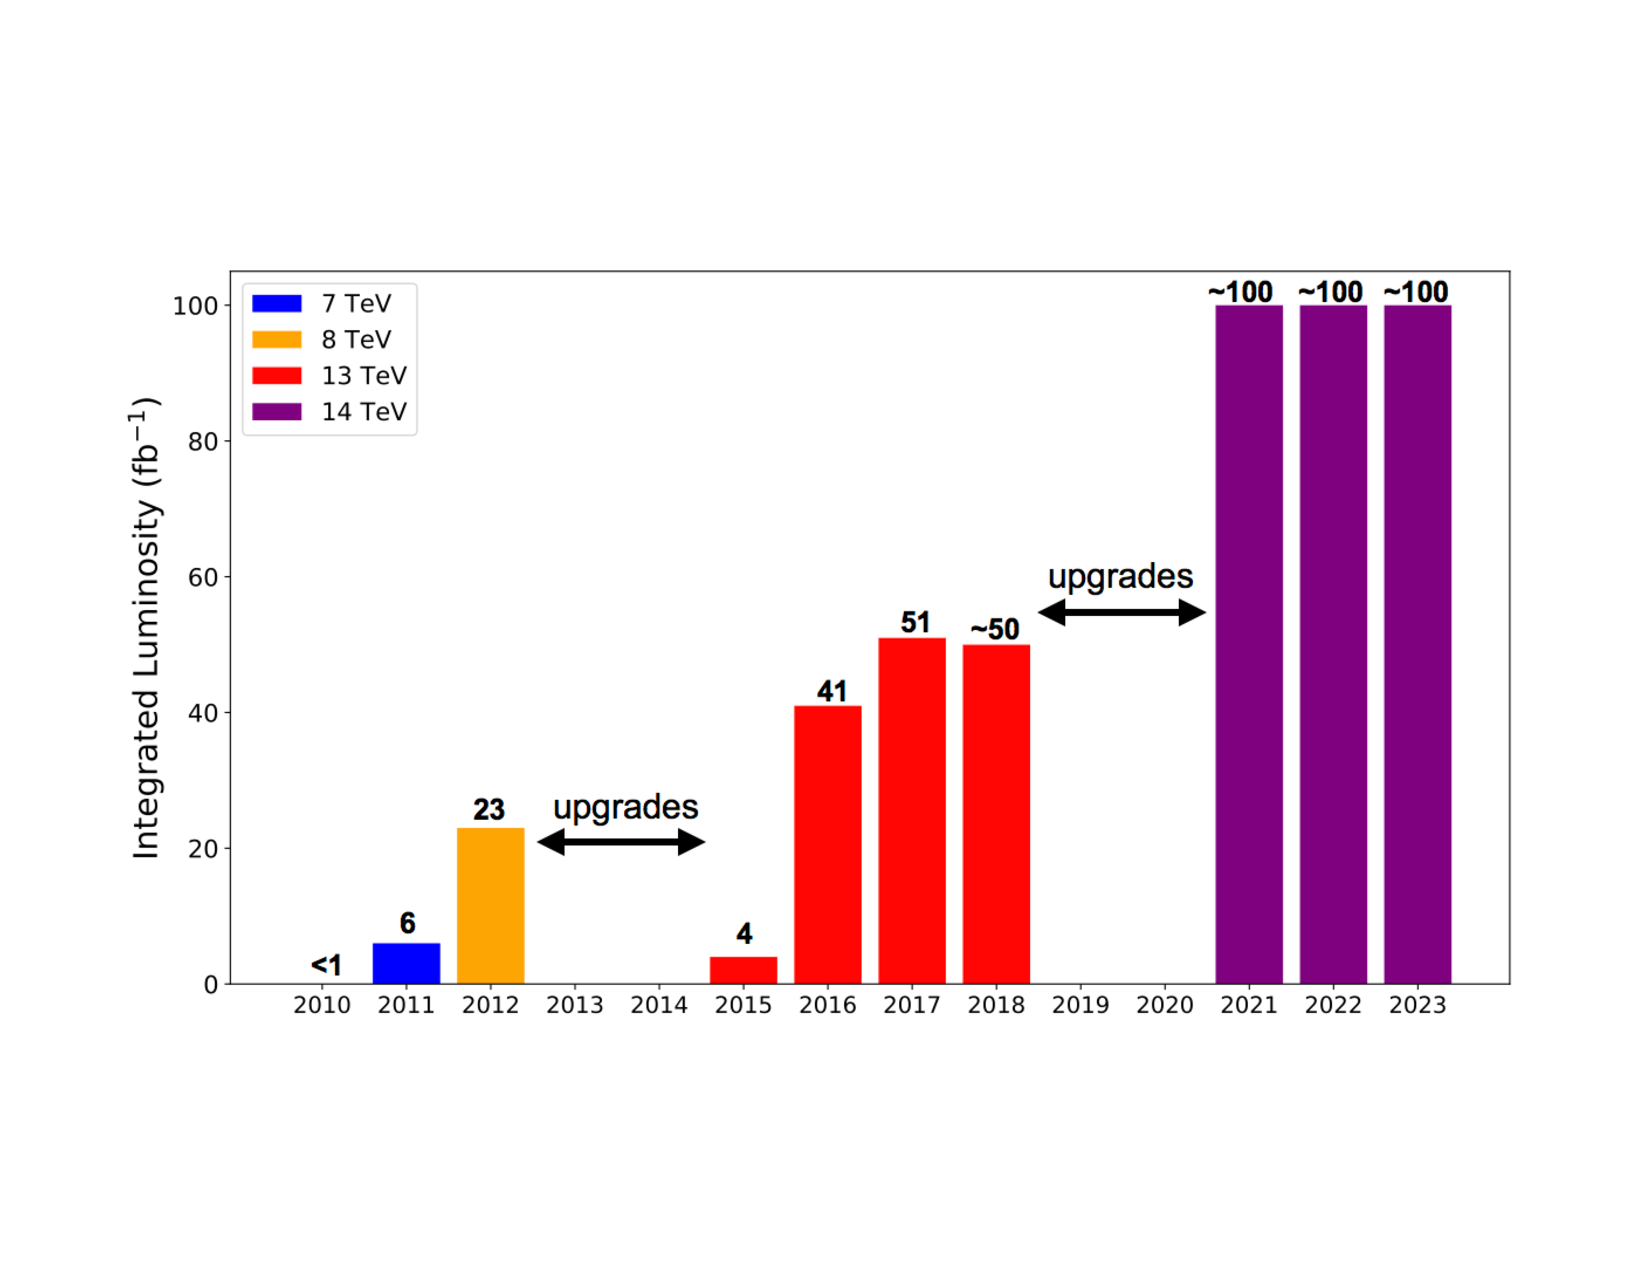
\includegraphics[angle=0,width=0.90\columnwidth]{fig/lhc_plan.pdf}
\end{center}
\caption{The (planned) integrated luminosity delivered and operating center-of-mass energy for the LHC from 2010-2023.}
\label{fig:lhc_plan}
\end{figure}

One physics object that is particularly difficult to measure is jets, as each jet is composed of roughly $\sim$10-100 correlated particles that are of various particle-types (charged hadrons, neutral hadrons, photons, etc), each with their own energy, and incident on many different detector channels.
All of these factors affect how well a detector measures a jet and thus contribute to a wide detector response for jets, where response is defined as
\begin{align}
\mathcal{R} = \frac{\pT^{\text{reconstructed}}}{\pT^{\text{true}}}.
\end{align}
By understanding how the jet response depends on these factors, jet measurements can be better corrected.
This can provide both better resolution for measurements, like those that reconstruct the Higgs mass from $\bbbar$ pairs, as well as better background-rejection for searches where, for example, events with mis-measured jets comprise the largest background.

Current methods~\cite{Khachatryan:2016kdb,Aaboud:2017jcu} only measure the jet response as a function of jet \pT and $\eta$, which are important first-order effects to consider.
Figure~\ref{fig:response_jeteta} shows that the mean response does vary with both variables, where the disjoint $\eta$-dependence is due to different detector technologies used at different values of $\eta$.
The main goal of measuring the jet response is to determine the mean of the response distribution correctly, as after correcting for this bias, jets will be measured correctly on average.
Figure~\ref{fig:nn_prediction} shows the jet response distribution (blue) and a model\footnotemark[1] of the distribution as a function of only jet \pT and $\eta$ (green, denoted \pT,$\eta$) overlaid and depicts the limitations of using only these variables:
While the green distribution does capture the mean of the blue distribution, it does not model much of the distribution's width, which results in a wide jet resolution for the detector.
Although much of this width is due to inherenty stochastic processes (e.g. photon production in scintillators), a question worth investigating is how much of jet response can be modeled by including the particle-level information of jets.

\begin{figure}[tbp!]
\begin{center}
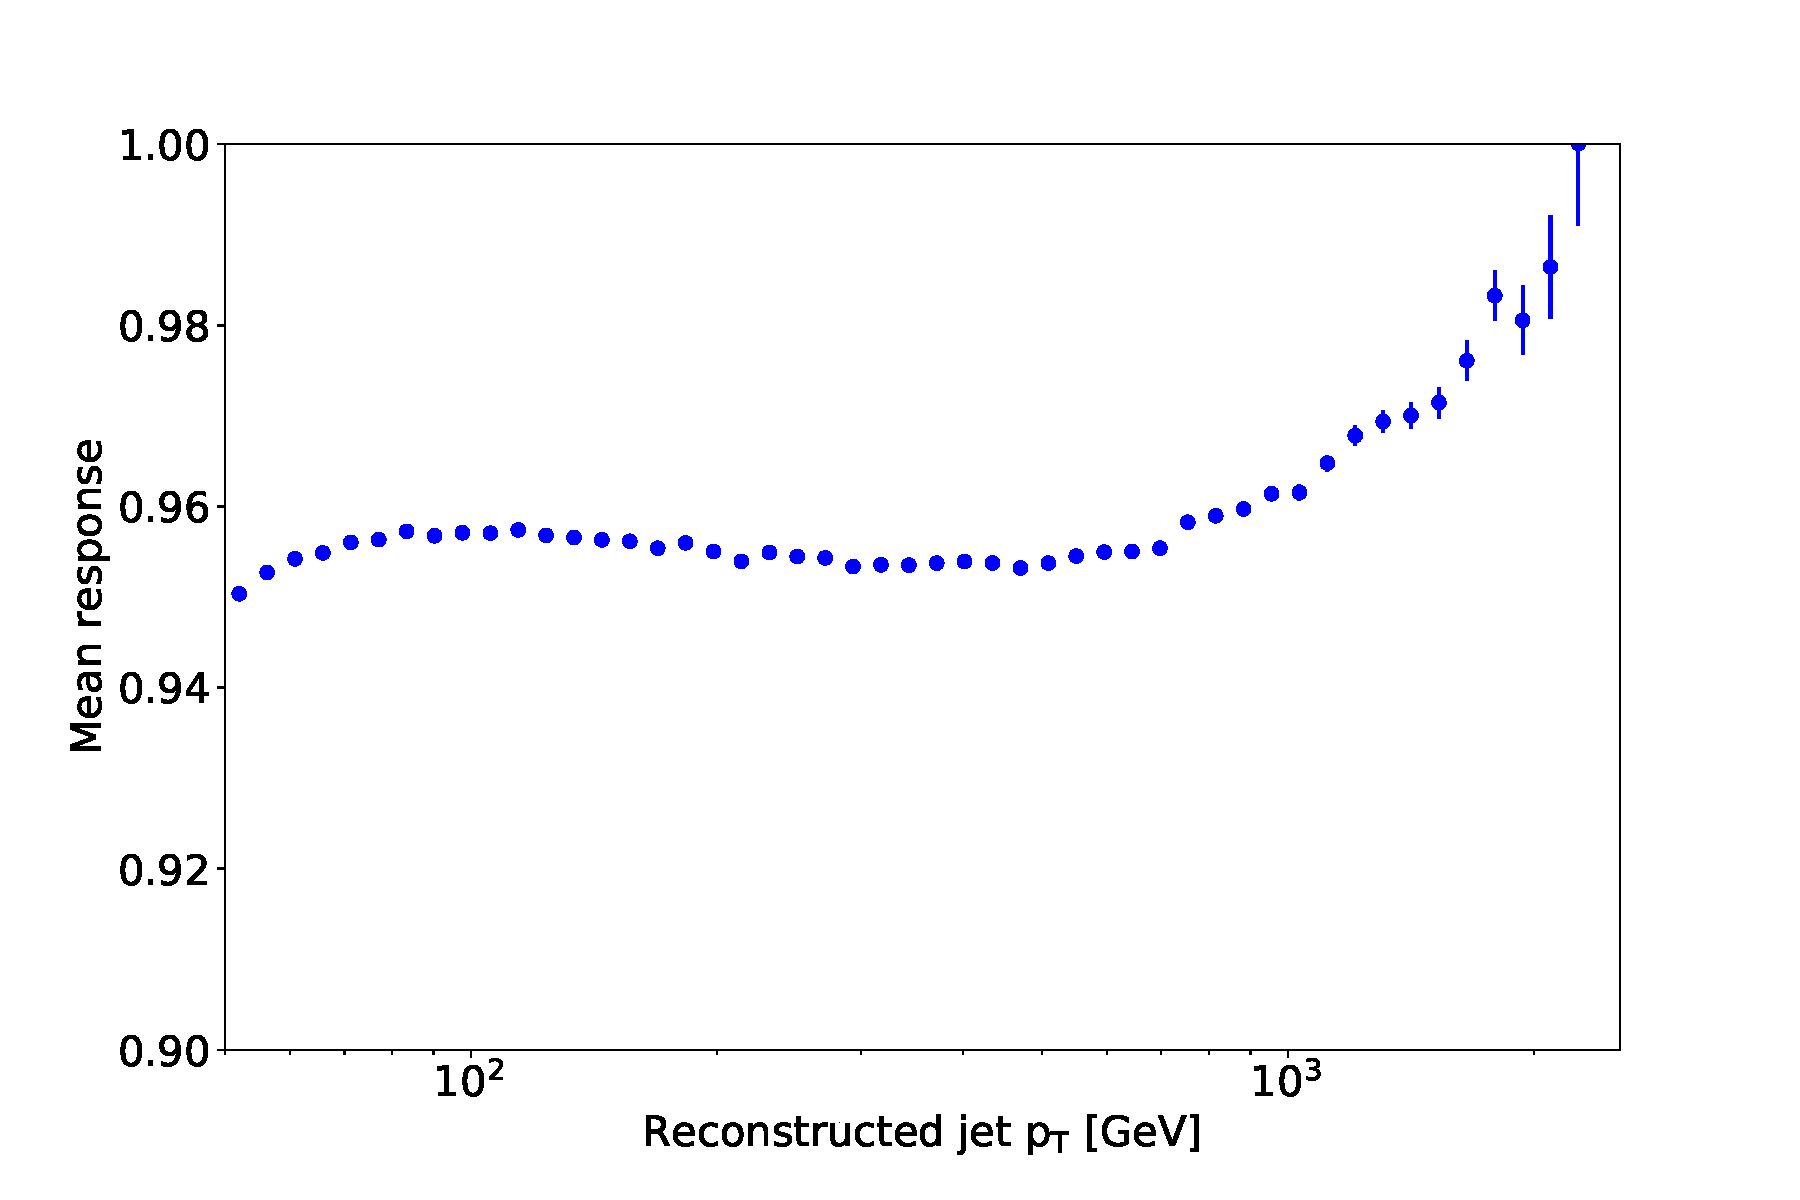
\includegraphics[angle=0,width=0.48\columnwidth]{fig/response_jetpt.pdf}
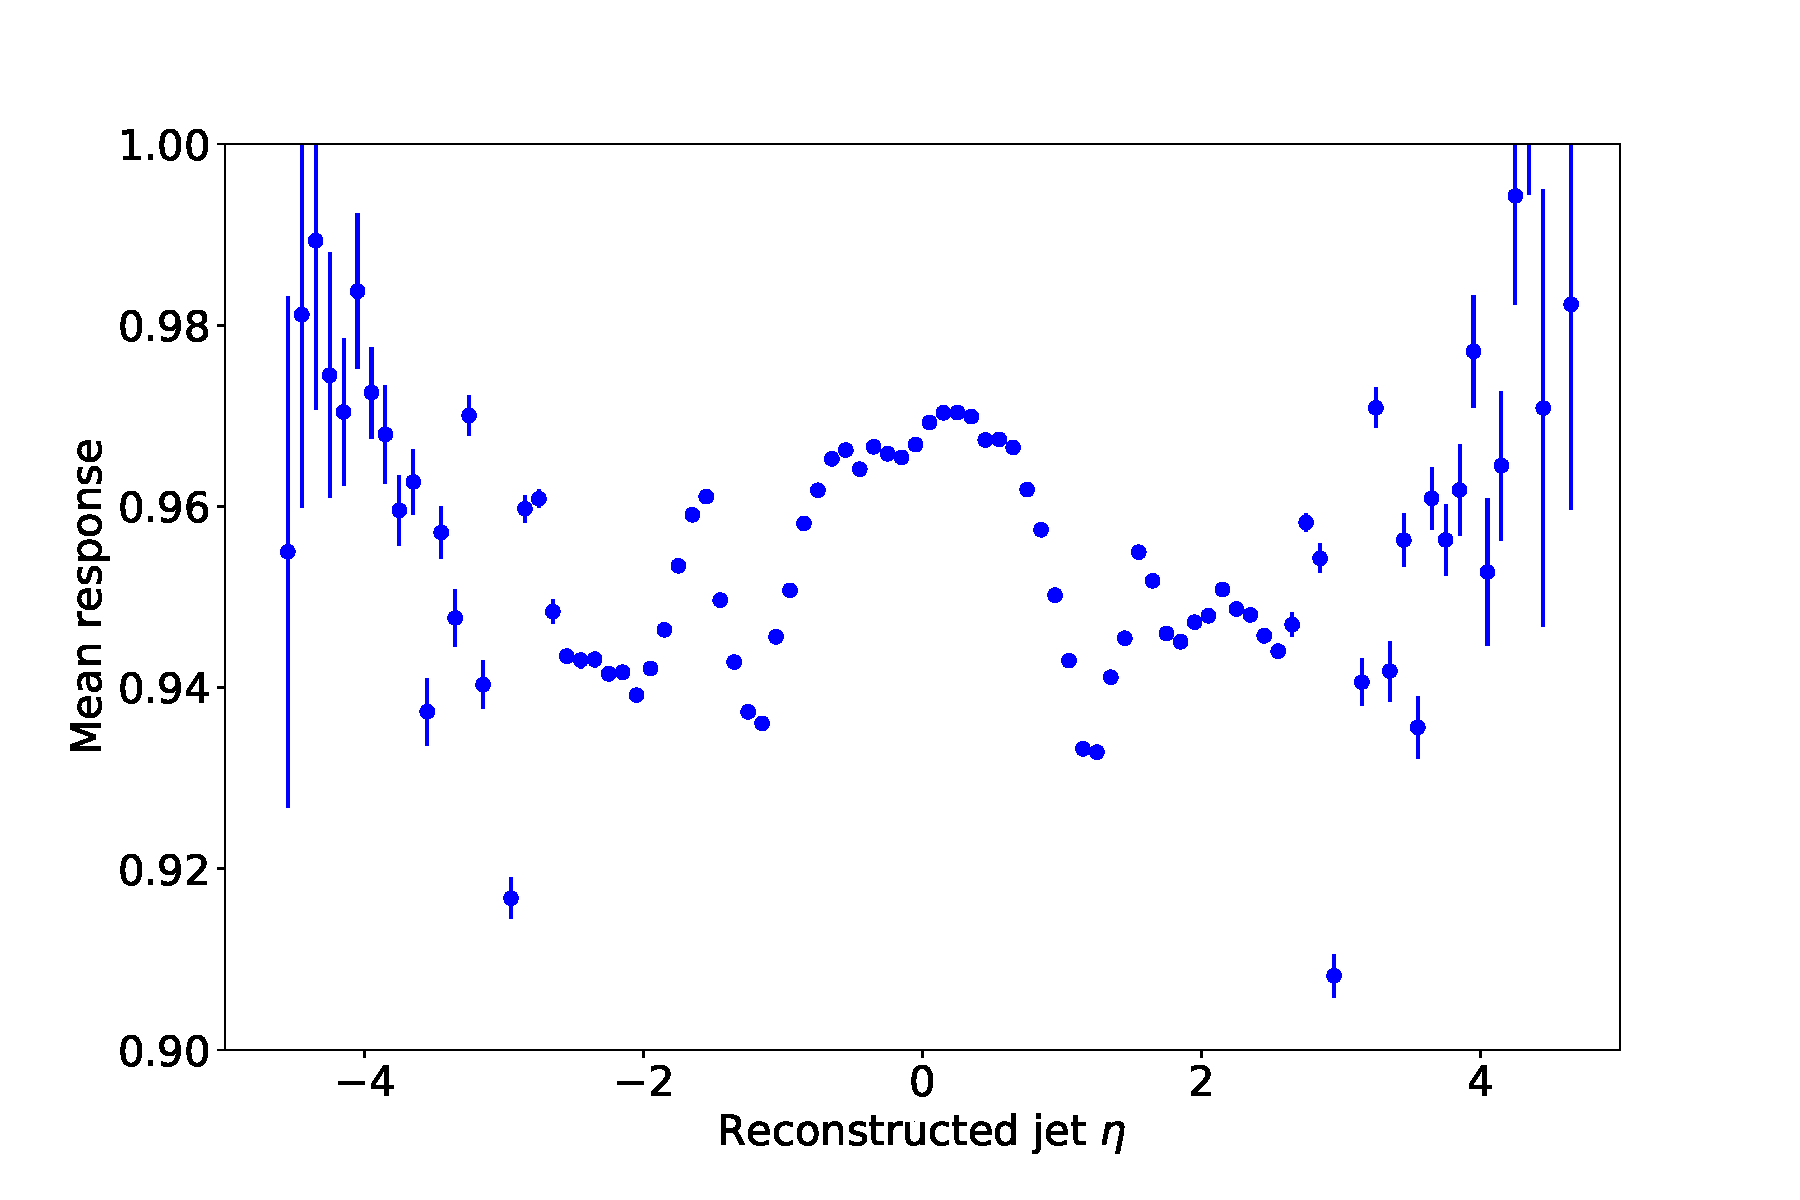
\includegraphics[angle=0,width=0.48\columnwidth]{fig/response_jeteta.pdf}
\end{center}
\caption{The mean jet response as a function of jet \pT (left) and $\eta$ (right).}
\label{fig:response_jeteta}
\end{figure}

\begin{figure}[tbp!]
\begin{center}
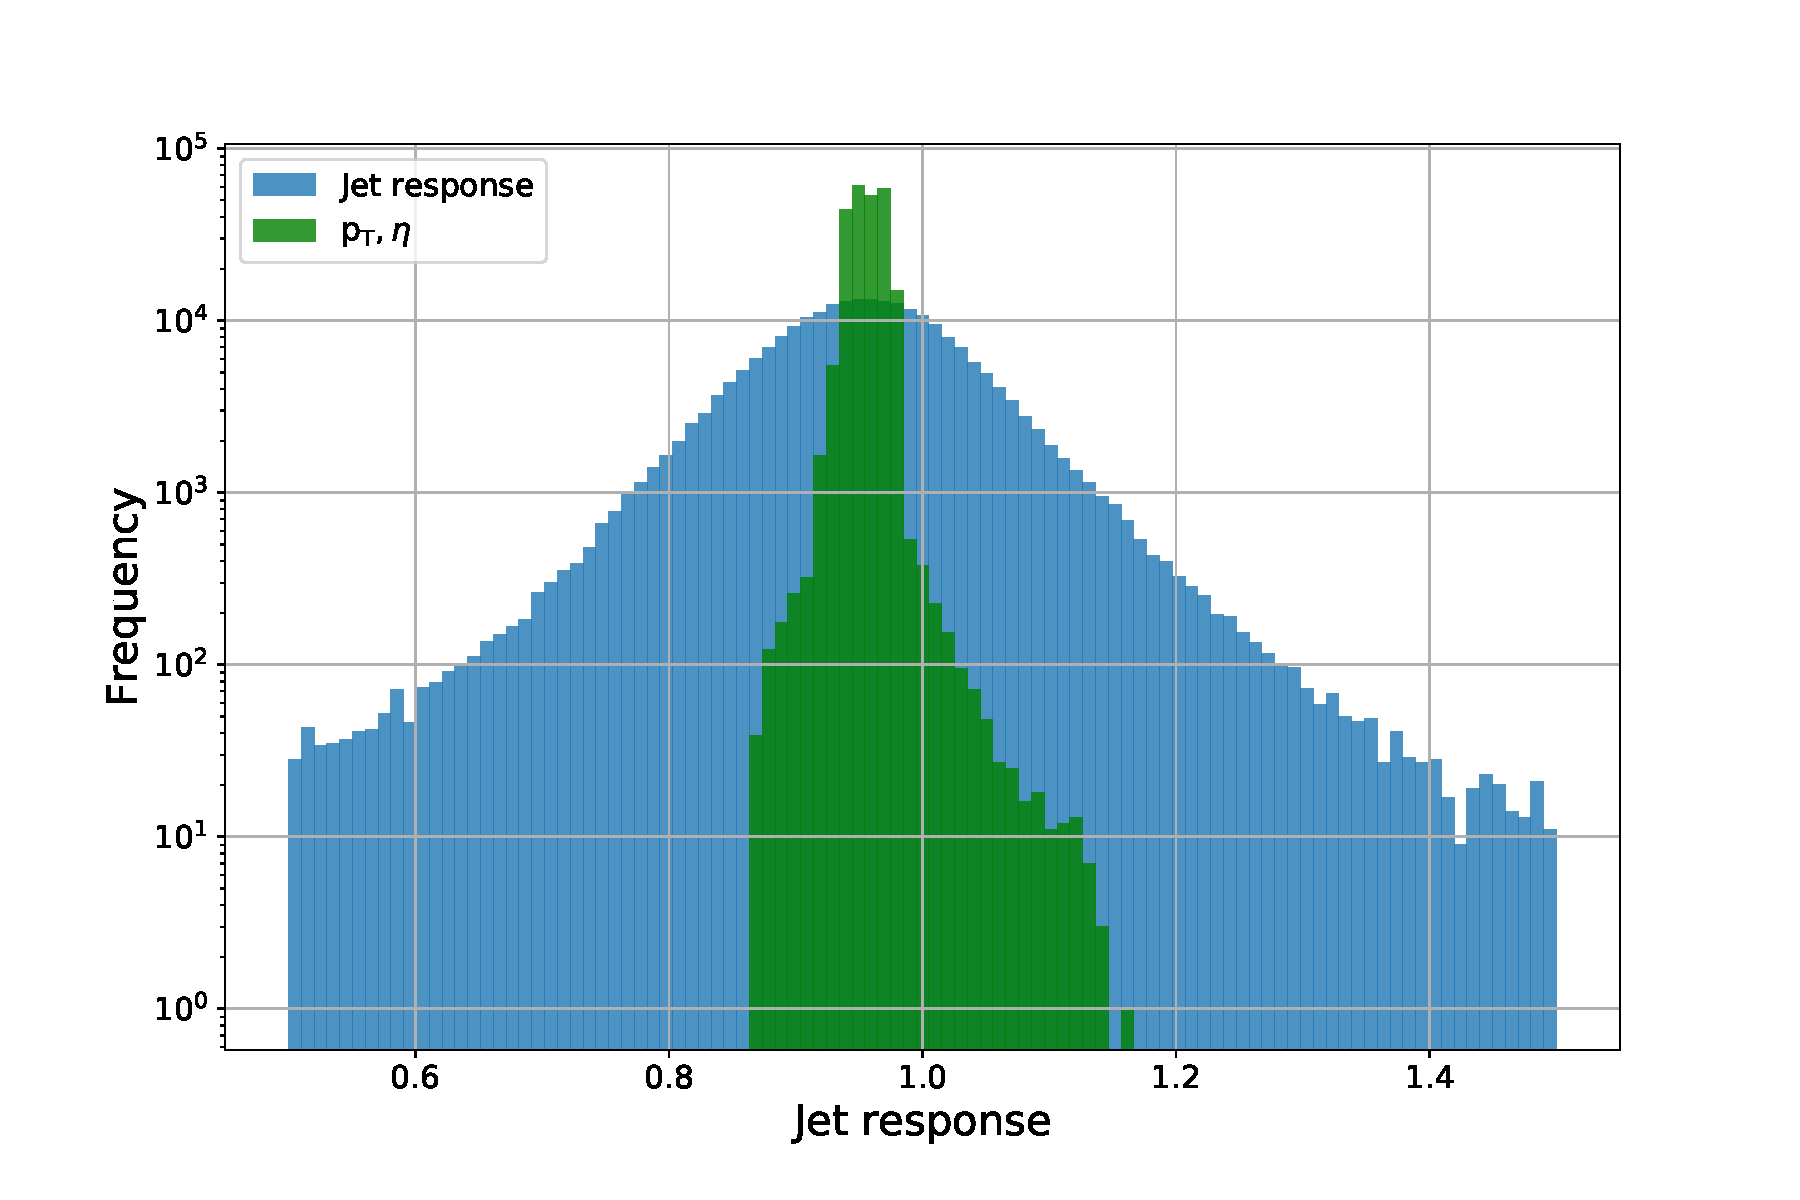
\includegraphics[angle=0,width=0.80\columnwidth]{fig/nn_prediction.pdf}
\end{center}
\caption{The true jet response distribution (blue) and a model of the response as a function of jet \pT and $\eta$ (green).}
\label{fig:nn_prediction}
\end{figure}

\footnotetext[1]{This model was generated by training a simple 3-hidden layer neural network with 32 hidden units each on only the jet \pT and $\eta$ with the jet response as the target.
The training and test set details are the same as those described in Section~\ref{sec:network_arch}.
The model complexity here far exceeds that which is necessary for a two-variable regression but is used for equal comparison to later results.}

\end{section}

\begin{section}{Jet Images}

One way to capture this particle-level information is by using the ``jet images'' technique~\cite{Cogan:2014oua,deOliveira:2015xxd}, which is a way of converting the detector signals of a jet into a 2D image that encodes this information.
Sophisticated image processing techniques can then be used on these images in order to extract the dependence of the detector response on the spatial and energy correlations of the jet fragmentation.
The use of jet images has been demonstrated to be effective for a variety of tasks, such as quark-gluon discrimination, W boson and top tagging, and in jet quenching studies with heavy-ion collisions~\cite{Cogan:2014oua,deOliveira:2015xxd,Barnard:2016qma,Kasieczka:2017nvn,Chien:2018dfn,Komiske:2016rsd}.

The process used in this study for generating is carried out for each jet in an event and is as follows:
\begin{itemize}
\item First, define a 2D histogram in $\eta$-$\phi$ space centered around the jet's $\eta$ and $\phi$. 
The exact binning choice is arbitrary, but it is helpful that the segmentation of the histogram approximates the segmentation of the detector and that the range of the axes depend on the radius of the jet clustring algorithm.
Here, for $R = 0.5$ jets, a range of two with 25 bins is used for both the $\eta$ and $\phi$ dimensions.
\item Next, fill the histogram based on the $\eta$ and $\phi$ of the constituent jet particles with the weight of each entry equal to the particle's \pT.
\item Finally, center the image such that the origin ($\eta = 0$, $\phi = 0$) corresponds to the highest \pT bin and normalize the image such that the value of the highest \pT bin equals one. 
\end{itemize}
Once completed, each bin of the histogram can be thought of as a ``pixel'' of an image with an intensity equal to the weight of that bin.
These images encode the particle-level spatial and energy information of a jet, and an example jet image is shown in Figure~\ref{fig:jetimage}.

\begin{figure}[tbp!]
\begin{center}
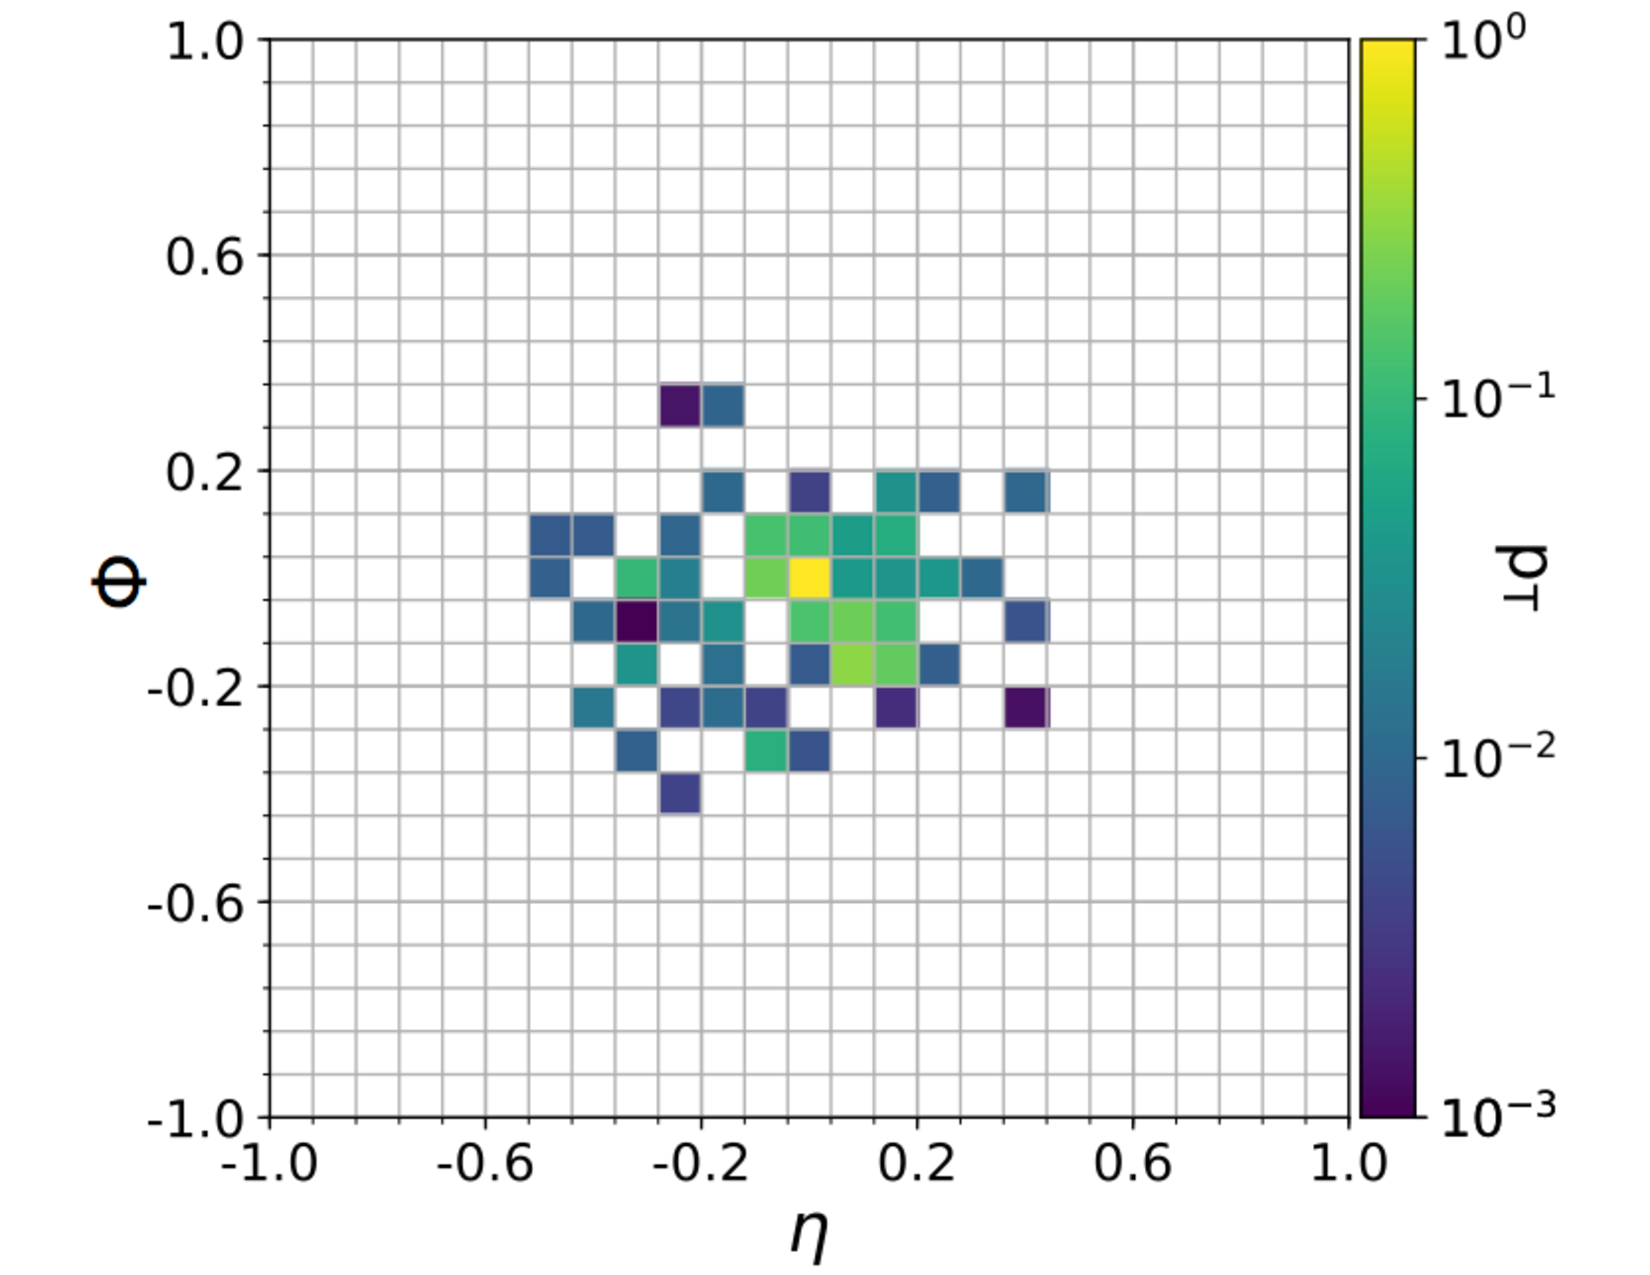
\includegraphics[angle=0,width=0.80\columnwidth]{fig/jetimage.pdf}
\end{center}
\caption{An example jet image.}
\label{fig:jetimage}
\end{figure}

Detectors, however, have different responses to different particles, and this information can be additionally encoded by splitting the jet images by particle type, where a separate jet image is constructed for each particle type. 
Figure~\ref{fig:jetimage_split} shows the example jet image now split into three categories: charged hadrons, neutral hadrons, and photons + electrons + muons (which is dominated by, and hereafter referred to as, photons).
The resulting three images can then be combined into a single 3-channel jet image, completely analagous to how a pixel encodes an R, G, and, B value in traditional colored images.
One can see that there is an information gain by comparing the average unnormalized jet images for each category, as shown in Figure~\ref{fig:jetimage_avg}.
For example, while subtle, it can be gleamed just by eye that the center of the average neutral hadron jet image is ``brighter'' than that of the average charged hadron image, which indicates that on average neutral hadrons are higher in \pT than are charged hadrons.
This information, along with other much lower-level information, is now made accessible.
The idea of ``colorizing'' jet images was first presented in Reference~\cite{Komiske:2016rsd}.

\begin{figure}[tbp!]
\begin{center}
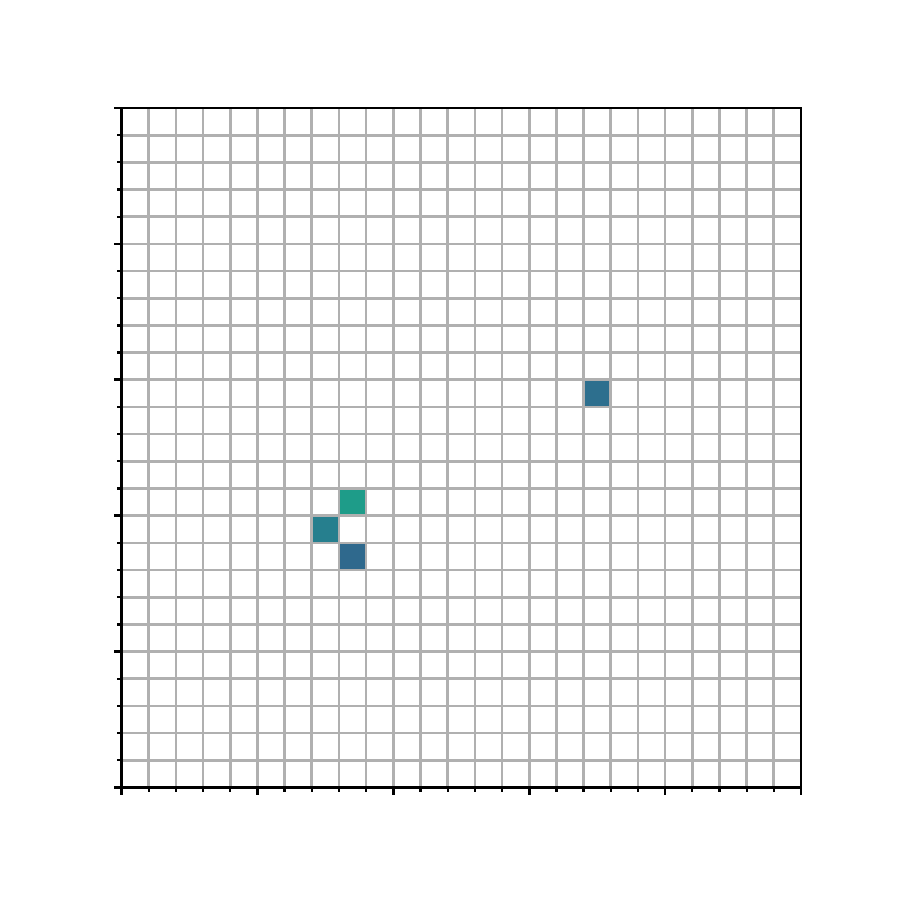
\includegraphics[angle=0,width=0.32\columnwidth]{fig/jetimage_ch.pdf}
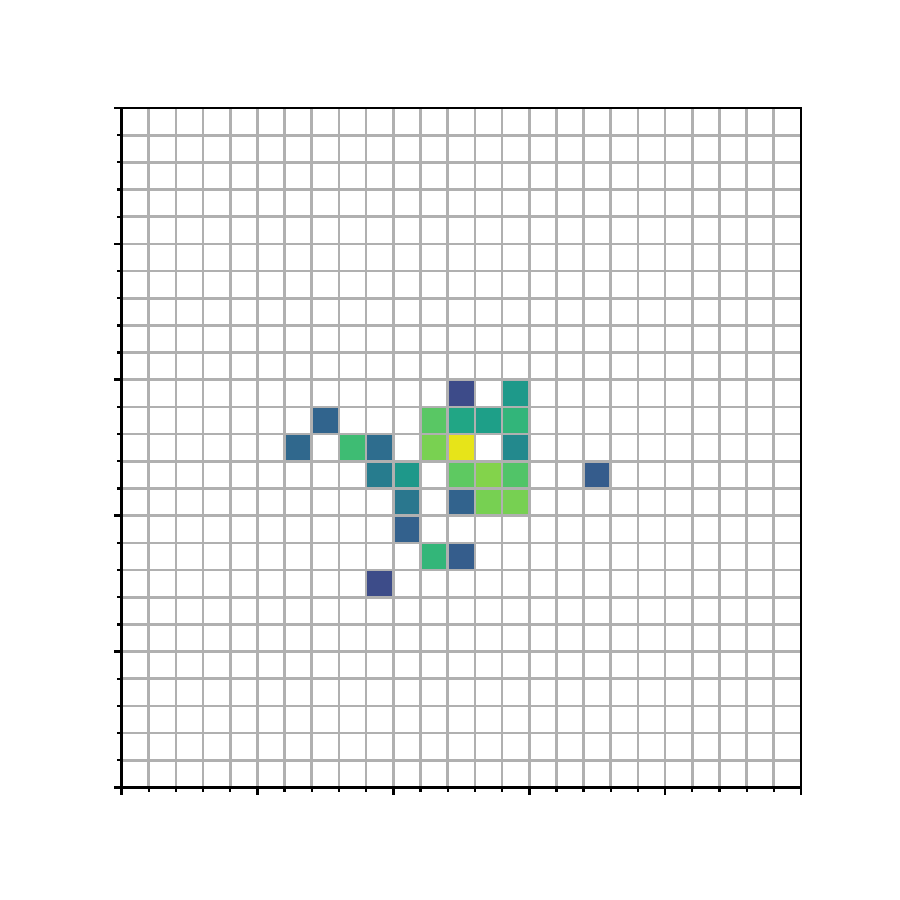
\includegraphics[angle=0,width=0.32\columnwidth]{fig/jetimage_nh.pdf}
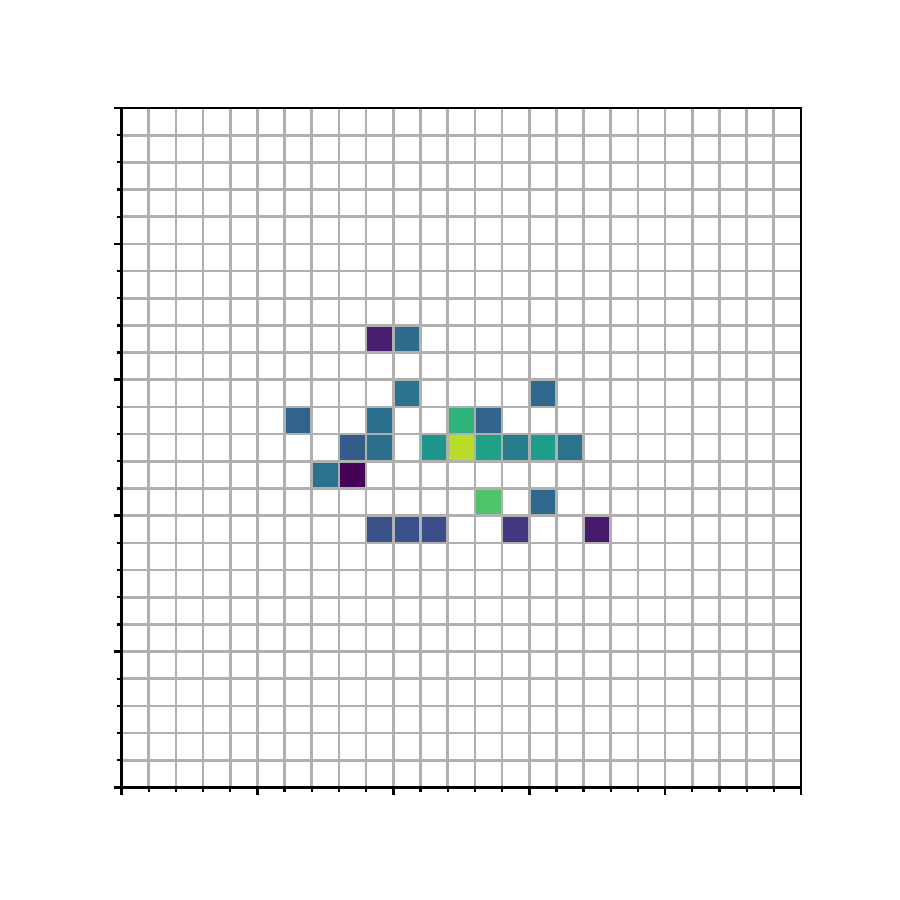
\includegraphics[angle=0,width=0.32\columnwidth]{fig/jetimage_ph.pdf}
\end{center}
\caption{The example jet image from Figure~\ref{fig:jetimage} split by particle type: charged hadrons (left), neutral hadrons (right), and photons + electrons + muons (right).}
\label{fig:jetimage_split}
\end{figure}

\begin{figure}[tbp!]
\begin{center}
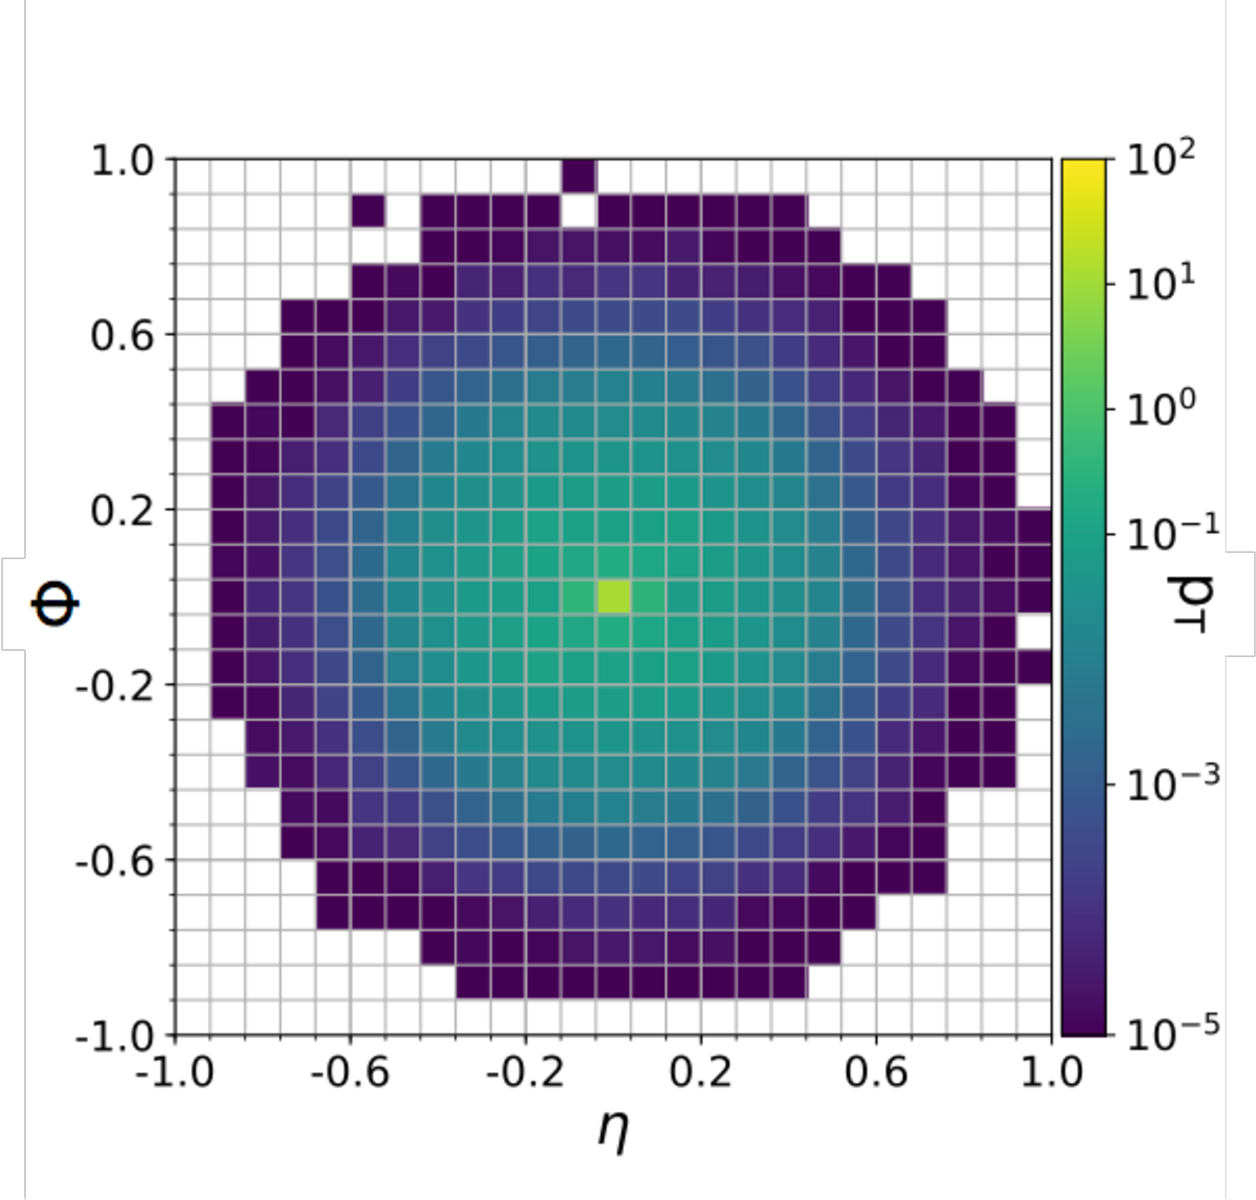
\includegraphics[angle=0,width=0.32\columnwidth]{fig/avgch_image.pdf}
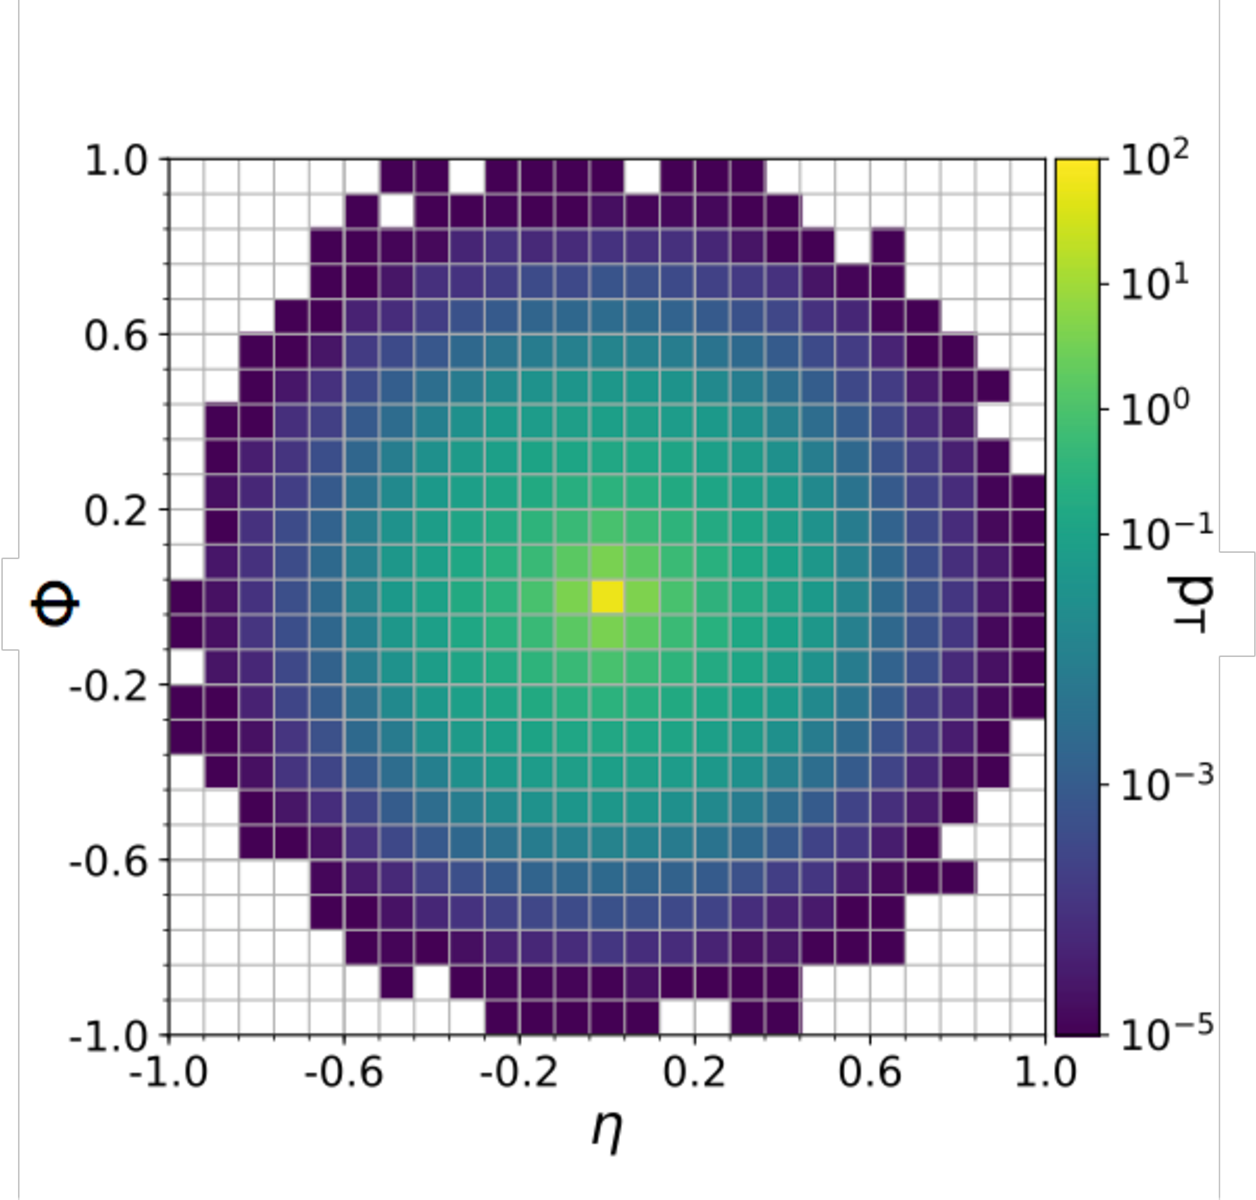
\includegraphics[angle=0,width=0.32\columnwidth]{fig/avgnh_image.pdf}
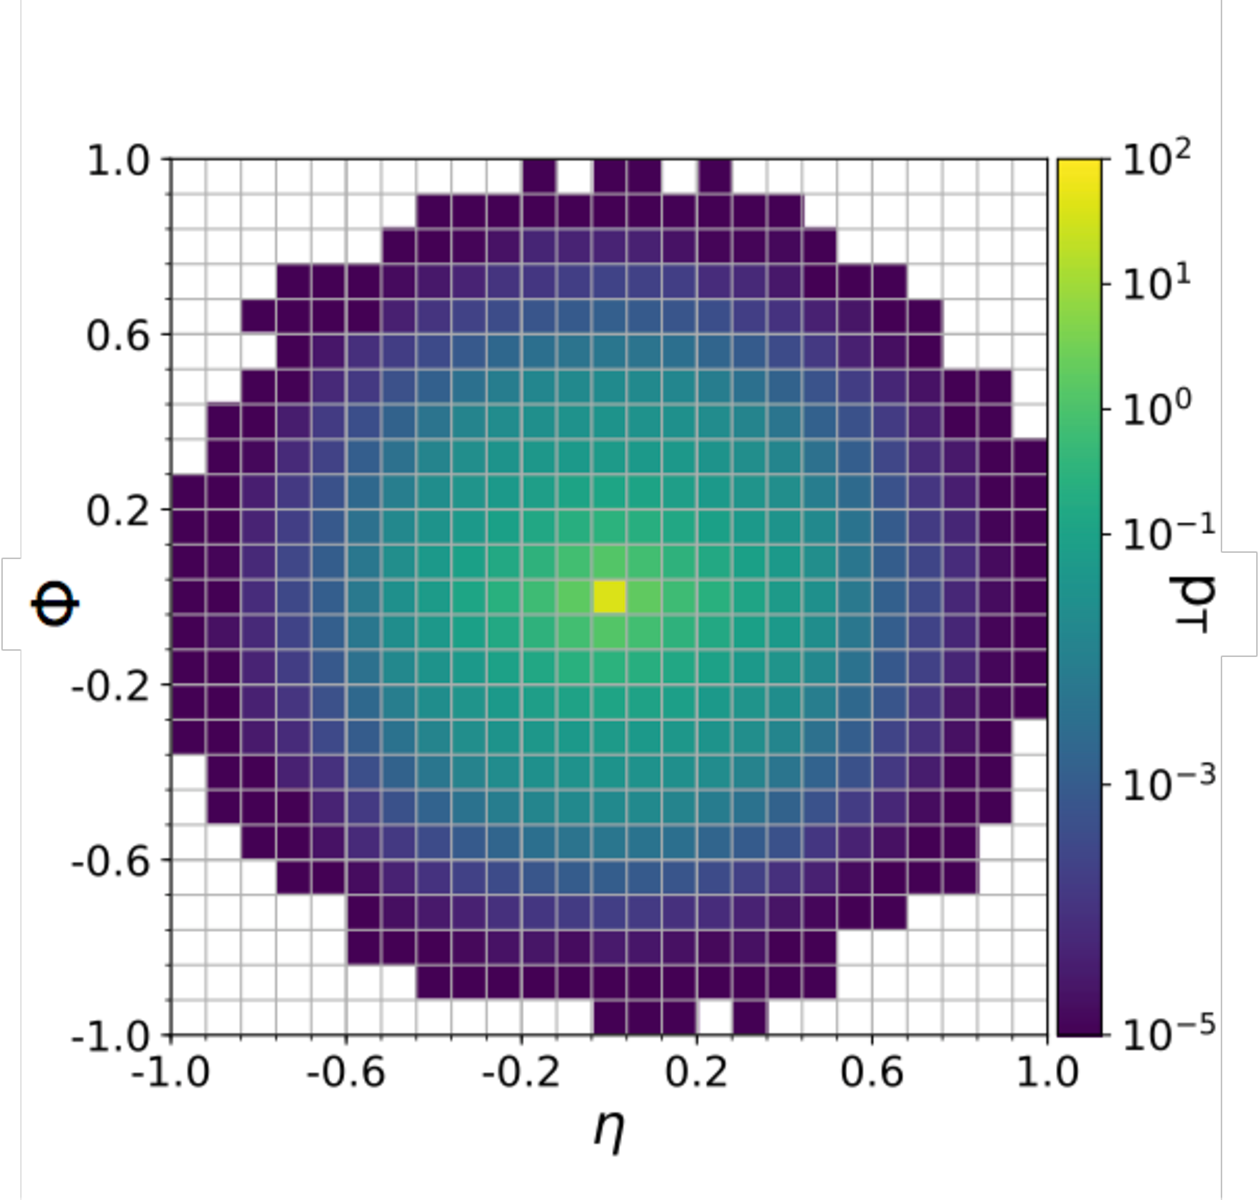
\includegraphics[angle=0,width=0.32\columnwidth]{fig/avgph_image.pdf}
\end{center}
\caption{Average unnormalized jet image for charged hadrons (left), neutral hadrons (right), and photons + electron + muons (right).}
\label{fig:jetimage_avg}
\end{figure}

\end{section}

\begin{section}{Network Architecture}
\label{sec:network_arch}

Now that jet images have been constructed that encode the particle-level jet information, the correlations between this information and the detector response needs to be extracted.
This can be done by training a deep convolutional neural network (CNN) and having it ``learn'' the jet response as a function of jet fragmentation.
The network architecture is composed of two main parts: a set of convolutional layers that are used as feature extractors and a set of fully-connected layers that build low-level features from those extracted by the convolutional layer.

Because these jet images are sparse, i.e. only 5-10\% of pixels are non-zero, the CNN architecture deviates from typical image processing heuristics.
For example, instead of standard 3x3 filters, the network uses relatively large filters in early layers in order to encapsulate more of the image and improve the network training.
Then, as the network reduces the image size through max-pooling layers, the filter sizes are correspondingly reduced, while increasing the number of filters in each layer to allow the network to learn many complex low-level features.

The exact network architecture is shown in Figure~\ref{fig:cnn_arch} and is detailed below:
\begin{itemize}
\item Input layer that accepts 25x25x3 jet images
\item Four convolution layers with $\tanh$ activations followed by 2x2 max-pooling layers
  \begin{itemize}
  \item 4 - 9x9 filters
  \item 8 - 6x6 filters
  \item 16 - 3x3 filters
  \item 32 - 1x1 filters
  \end{itemize}
\item Flatten and merge jet \pT and $\eta$ features
\item Three fully connected layers, each with 32 hidden-units, ReLu activations, and 10\% dropout
\item Output layer with linear activation that outputs the predicted jet response
\end{itemize}

\begin{figure}[tbp!]
\begin{center}
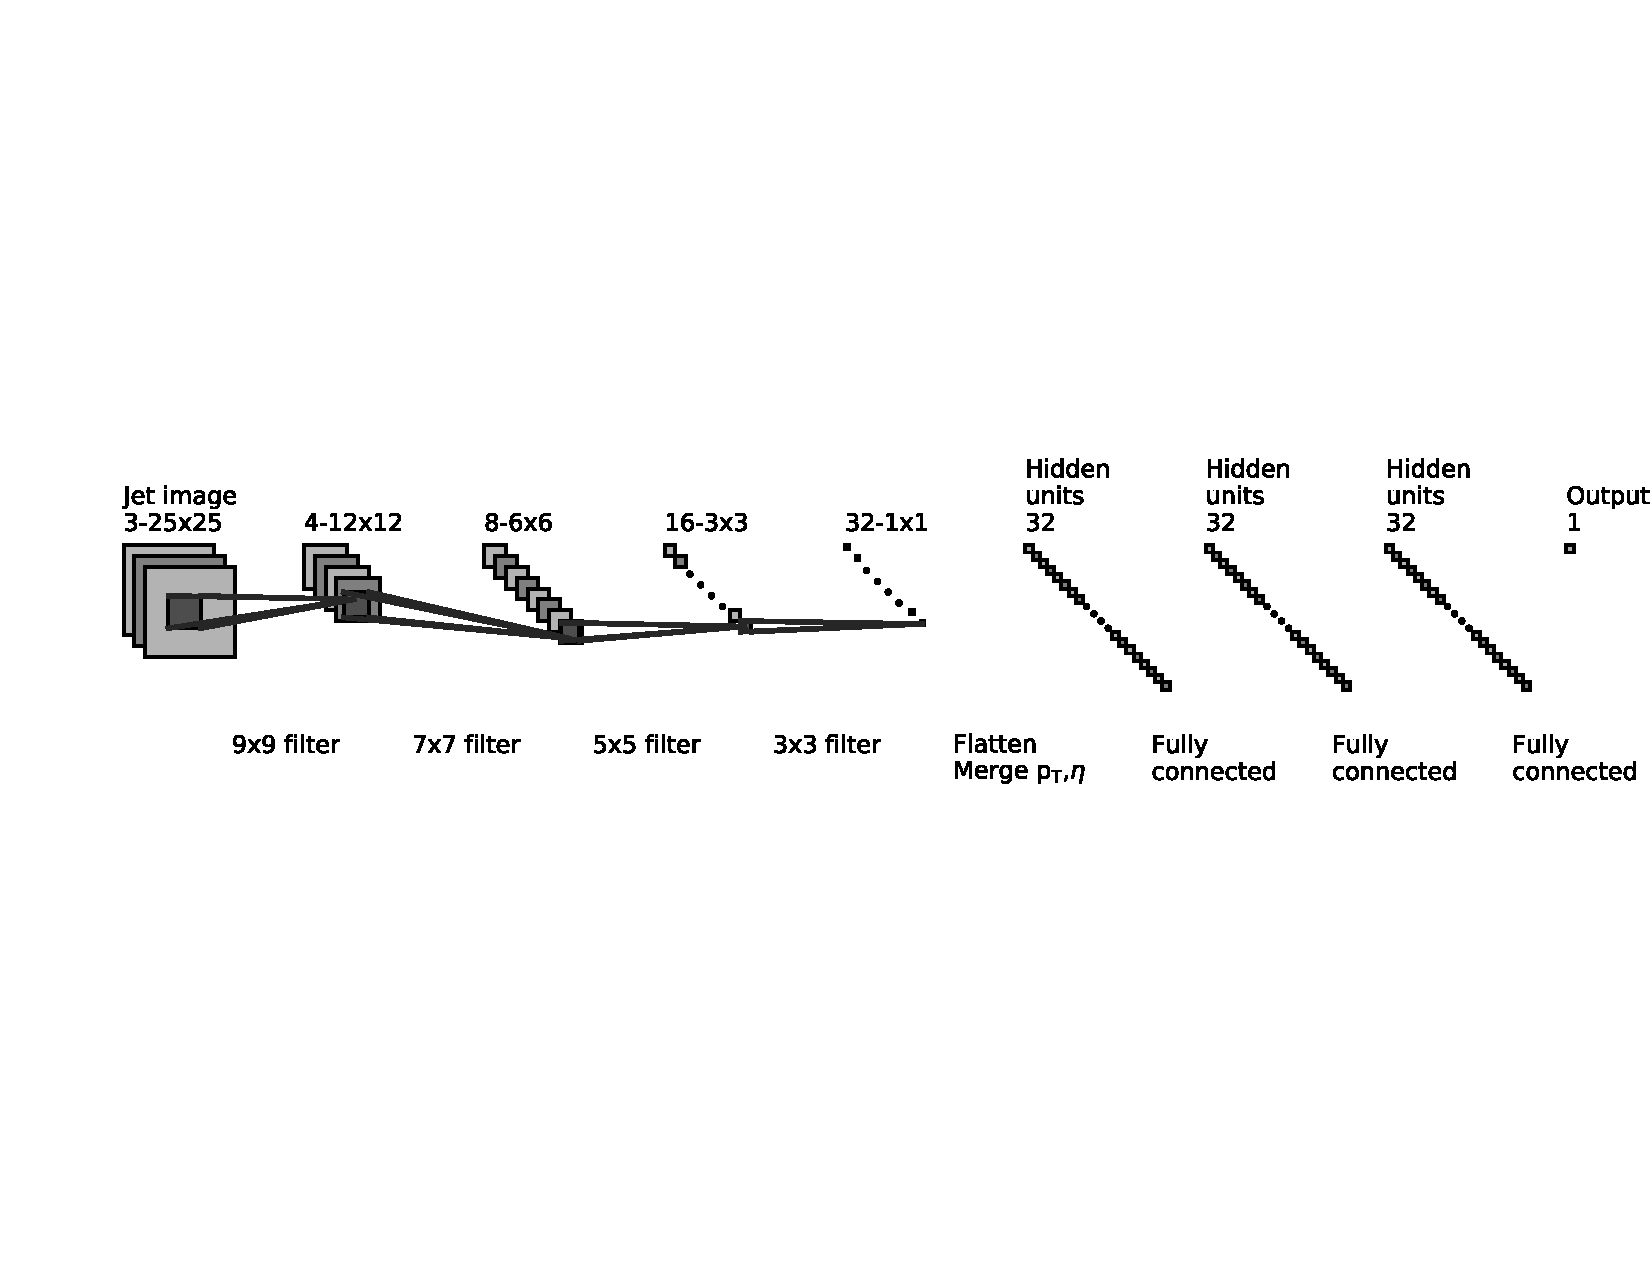
\includegraphics[angle=0,width=0.95\columnwidth]{fig/cnn_arch.pdf}
\end{center}
\caption{Schematic of the convolutional neural network architecture.}
\label{fig:cnn_arch}
\end{figure}

The network is trained using $\sim$2 million jets and tested on $\sim$200,000 jets. 
These jets are taken from a 2012, $\sqrt{s} = 8~\TeV$ simulation of QCD events obtained from CMS Open Data~\cite{cms_opendata} that does not include pileup interactions.
Jets in this sample are formed using the anti-\kT clustering algorithm with $R = 0.5$ and are selected by requiring they have $\pT > 50~\GeV$.
The mean squared error (MSE) loss function is optimized with the ADAM optimizer (learning rate = 0.001, $\beta_1 = 0.9$, $\beta_2 = 0.999$) using stochastic gradient descent with a batch size of 256.

\end{section}

\begin{section}{Results}

The results from the training of this network are presented in Figure~\ref{fig:cnn_prediction} which shows the true jet response distribution of the test set (blue) and the corresponding predictions of the \pT,$\eta$ model (green) and the CNN model (orange, denoted \pT,$\eta$ + image).
In this figure, one can see that the CNN is able to capture a wider range of the jet response, corresponding to a $\sim$10\% improvement with respect to the MSE.
Thus, one can see that the jet images not only contain extra relevant information but also that the CNN is able to extract it.
One things of note is that the CNN seems to model the high-response tail better than the low-response tail.
This behavior is not yet fully understood but believed to be due to biases in the jet selection of the training set.

\begin{figure}[tbp!]
\begin{center}
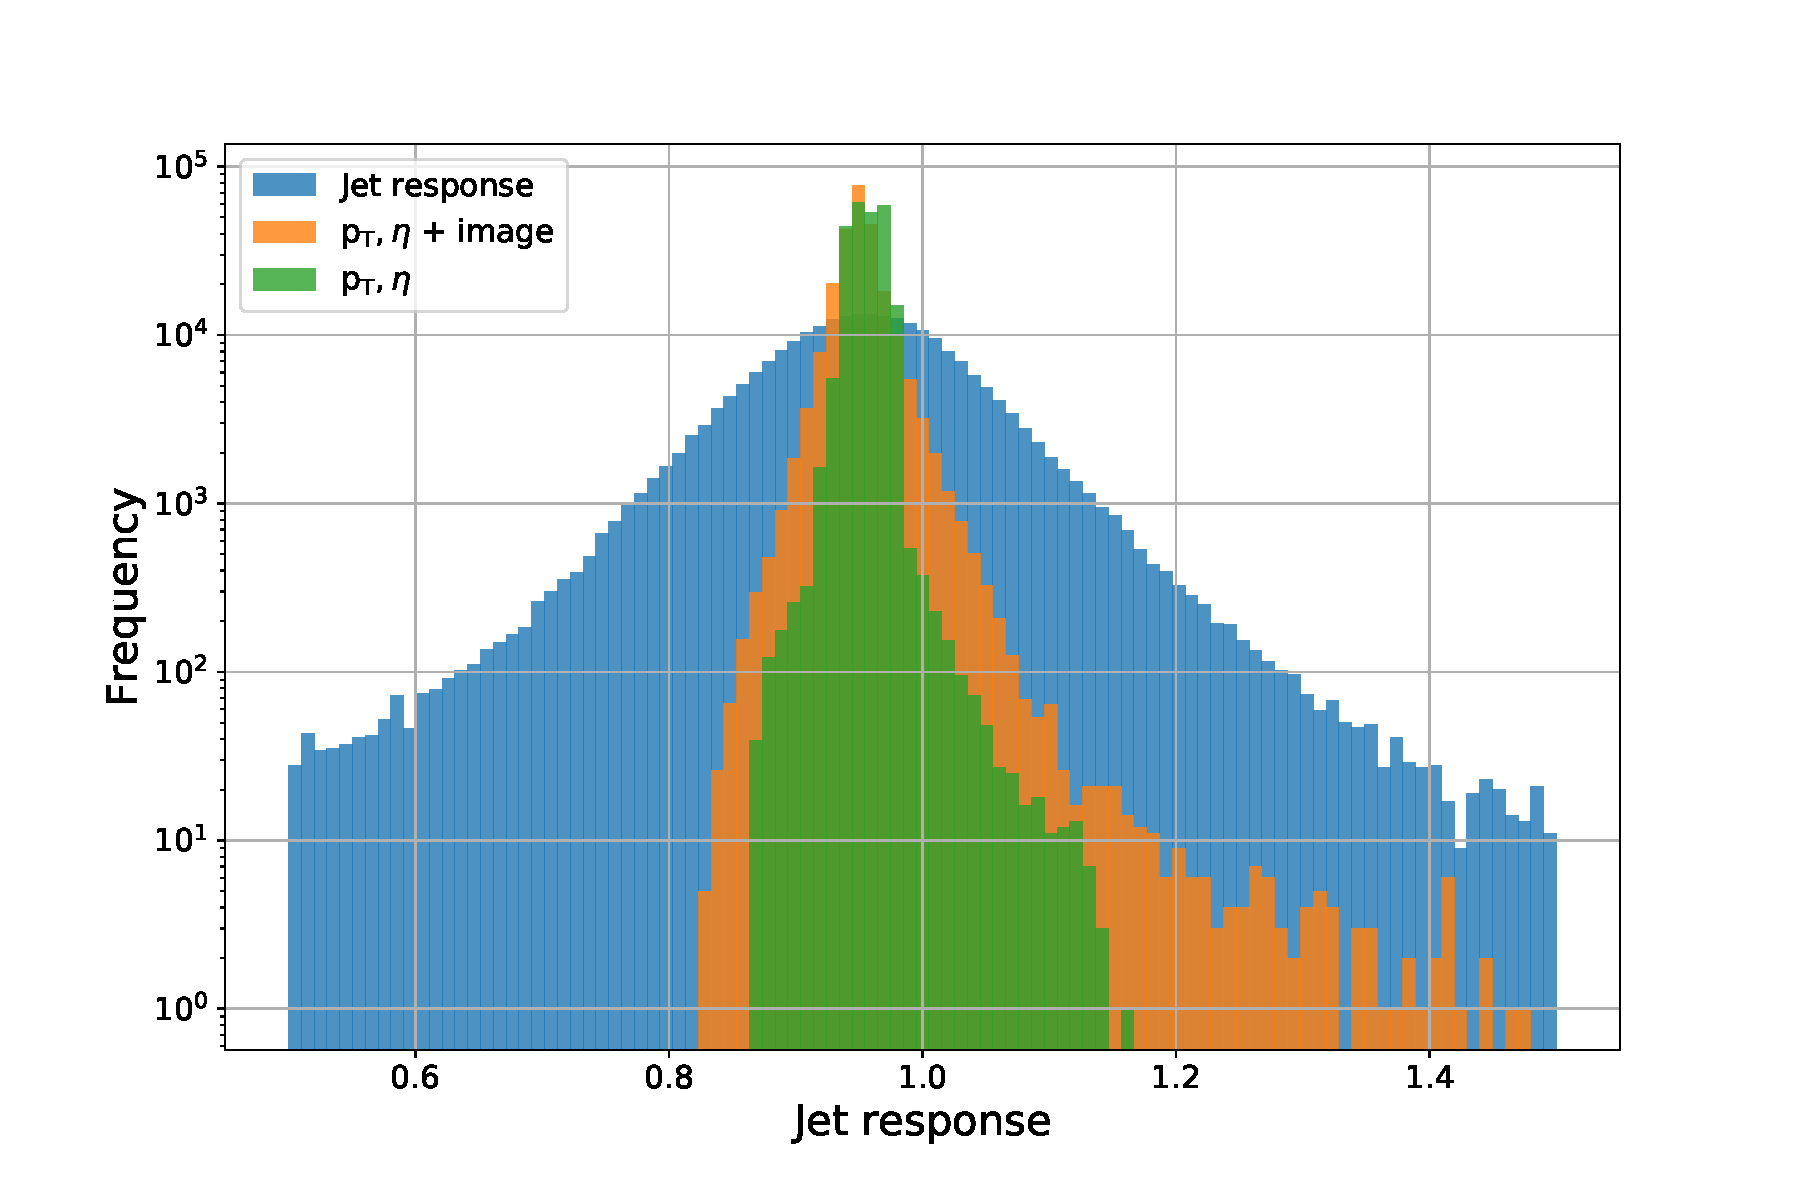
\includegraphics[angle=0,width=0.80\columnwidth]{fig/cnn_prediction.pdf}
\end{center}
\caption{The true jet response distribution (blue), a model of the response trained only on jet \pT and $\eta$ (green), and a model of the response additionally trained with jet images (orange).}
\label{fig:cnn_prediction}
\end{figure}

One way to see what the CNN is learning is by examining the response is modeled as a function of particle-type.
Figure~\ref{fig:response_energyfrac} shows the mean response in bins of fractional jet energy due to charged hadrons (left), neutral hadrons (middle), and photons (right).
The mean response of the model using only \pT and $\eta$, depicted in green data points, is flat as a function of jet energy in each of the plots, which is expected because the network was not given any information about particle type.
The mean response of the CNN model (orange), however, is starting to show the same dependencies on particle type as the true jet response (blue).
It is believed that with a larger training set this modelling will improve further.

\begin{figure}[tbp!]
\begin{center}
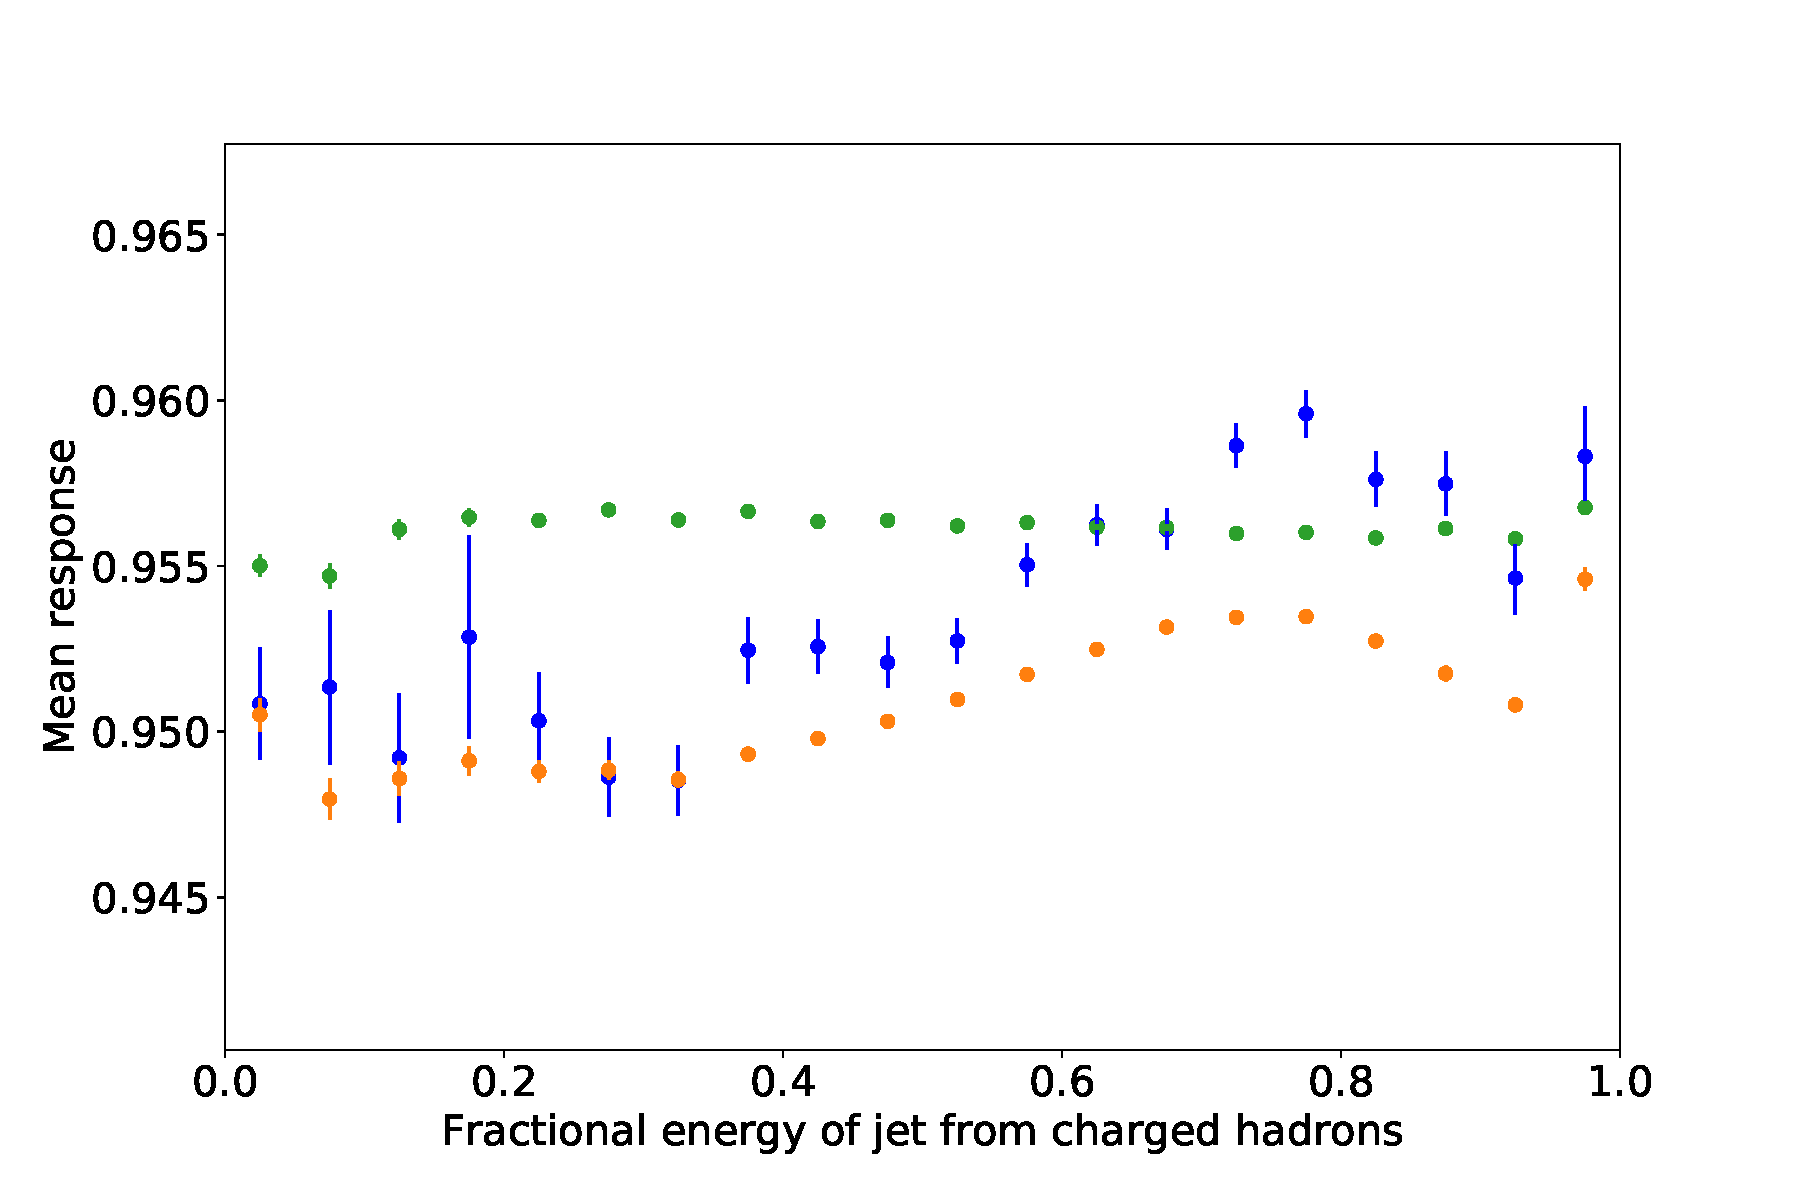
\includegraphics[angle=0,width=0.32\columnwidth]{fig/response_chf.pdf}
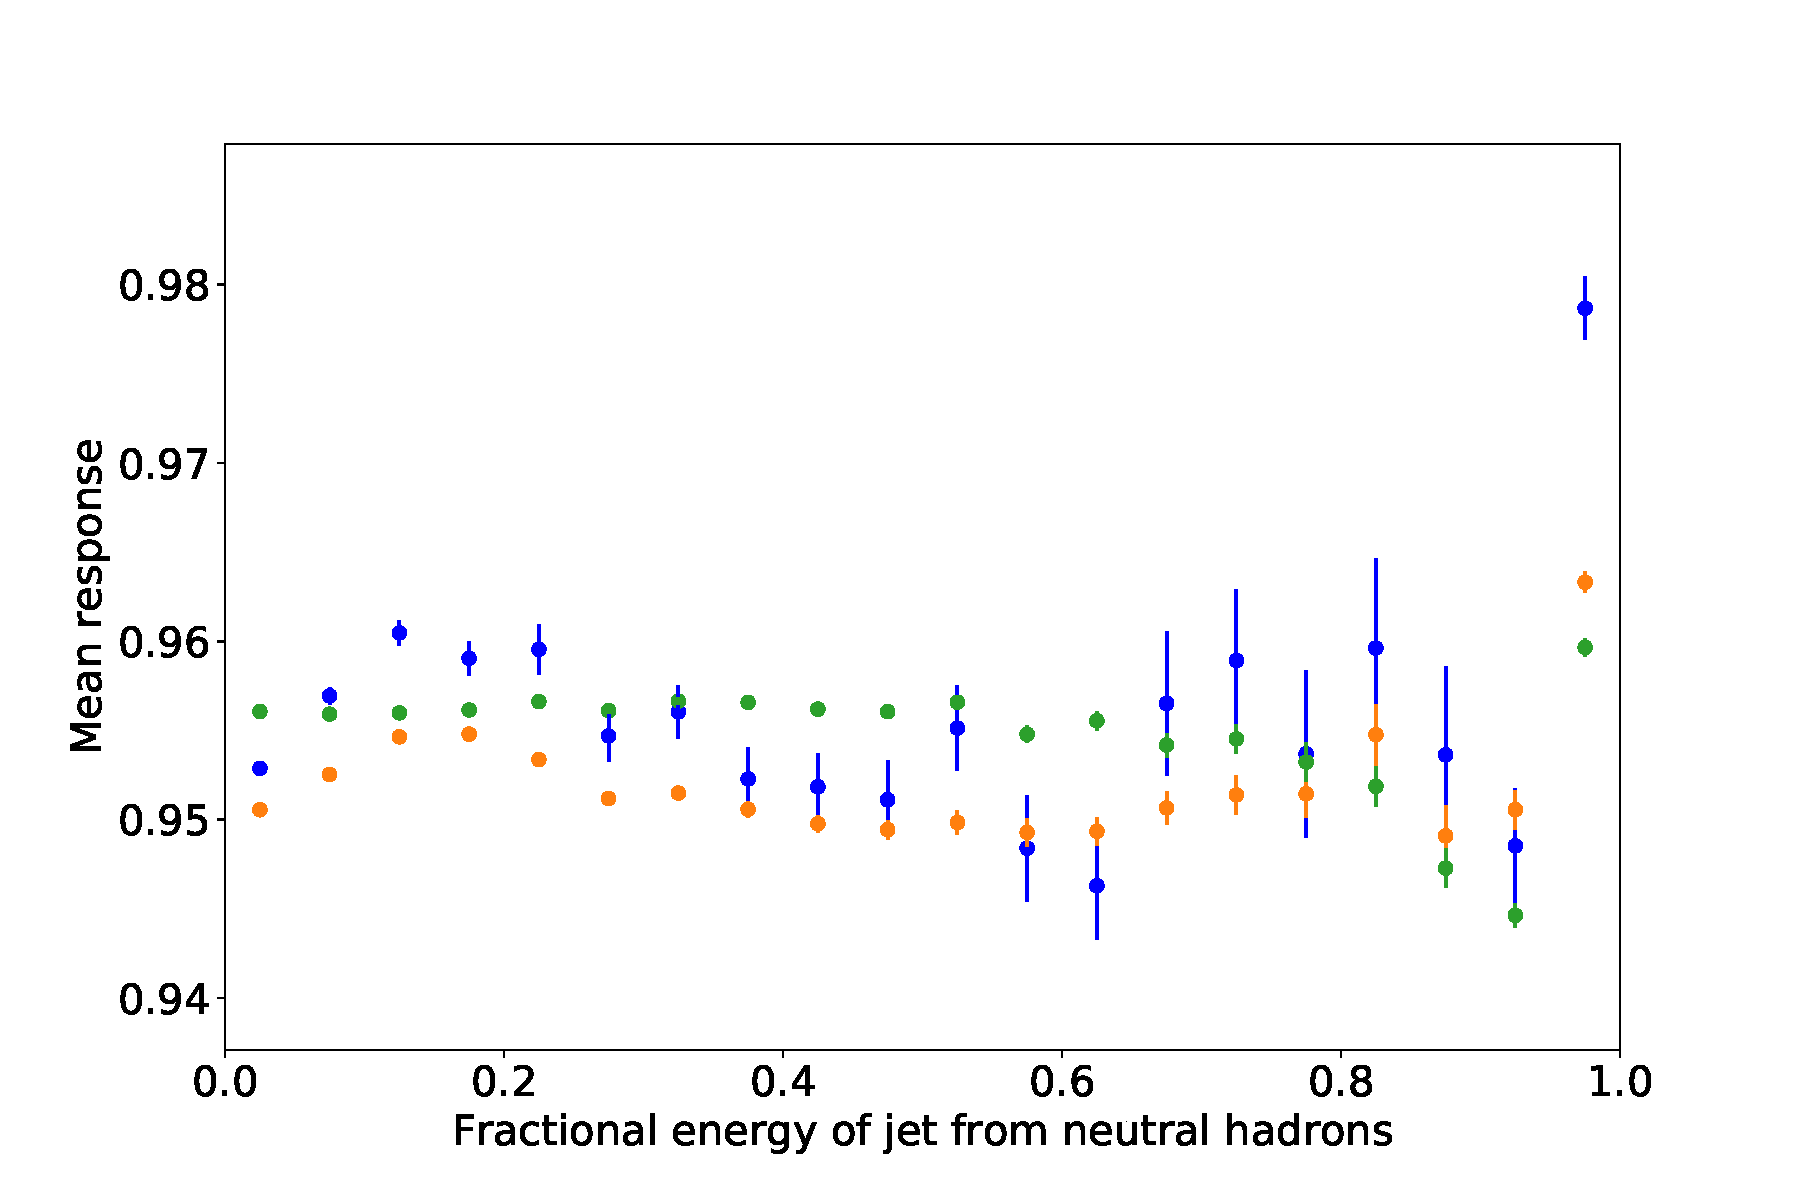
\includegraphics[angle=0,width=0.32\columnwidth]{fig/response_nhf.pdf}
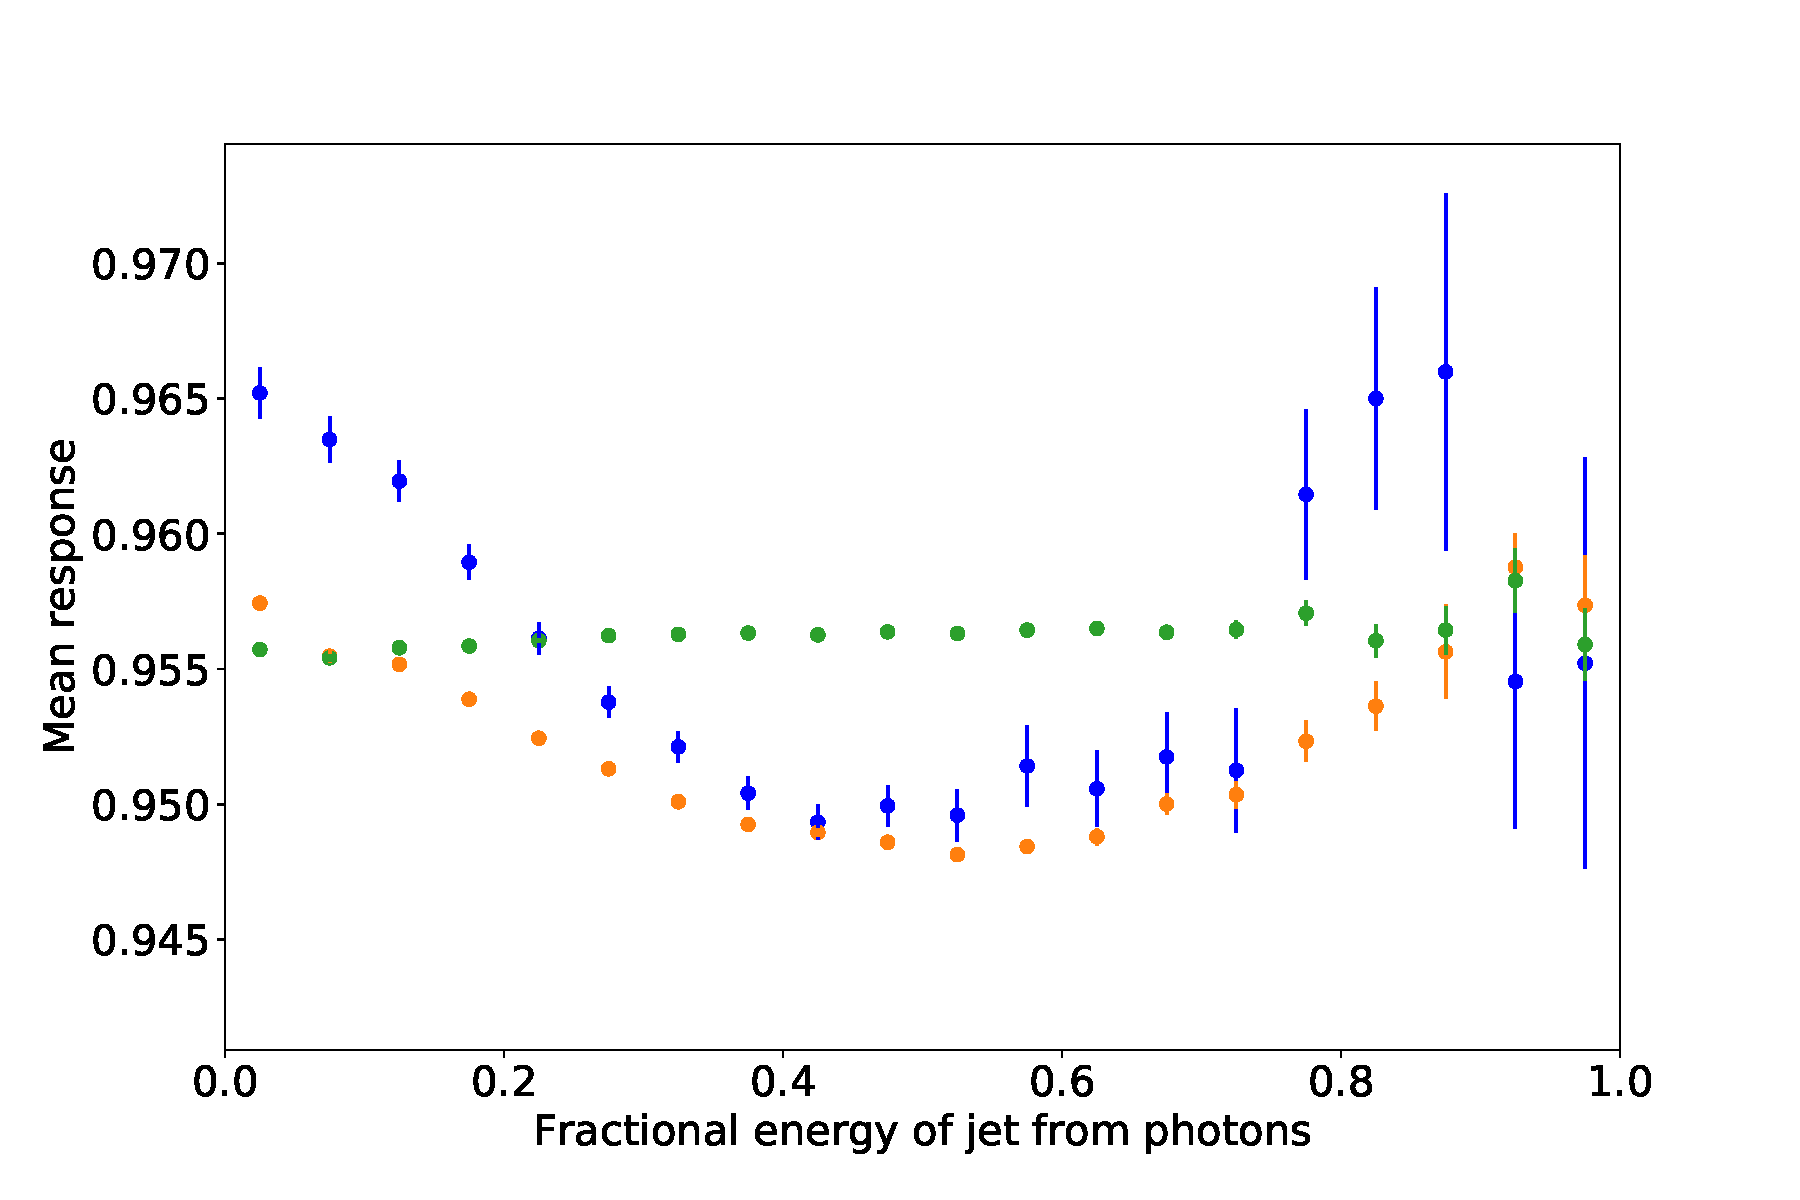
\includegraphics[angle=0,width=0.32\columnwidth]{fig/response_phf.pdf}
\end{center}
\caption{The mean jet response as a function of the fractional jet energy from charged hadrons (left), neutral hadrons (middle), and photons + electrons + muons (right).}
\label{fig:response_energyfrac}
\end{figure}

At this point, one may wonder how much of this improvement is due to the jet images versus the network simply having more information.
To separate the two effects, a dense neural network (corresponding to just the fully connected portion of the CNN network) is trained in which information on the jet fragmentation is included, i.e. the multiplicity and fractional jet energy of the particle types.
This model, shown as the purple distribution in Figure~\ref{fig:dnn_prediction}, is able to explain only roughly half the improvement of the model trained on jet images, as it improves over the \pT,$\eta$ model by about ~5\% with respect to the MSE.
Thus, it appears that the spatial and energy correlations encoded in jet images carry additional informationimportant for predicting the jet response.

\begin{figure}[tbp!]
\begin{center}
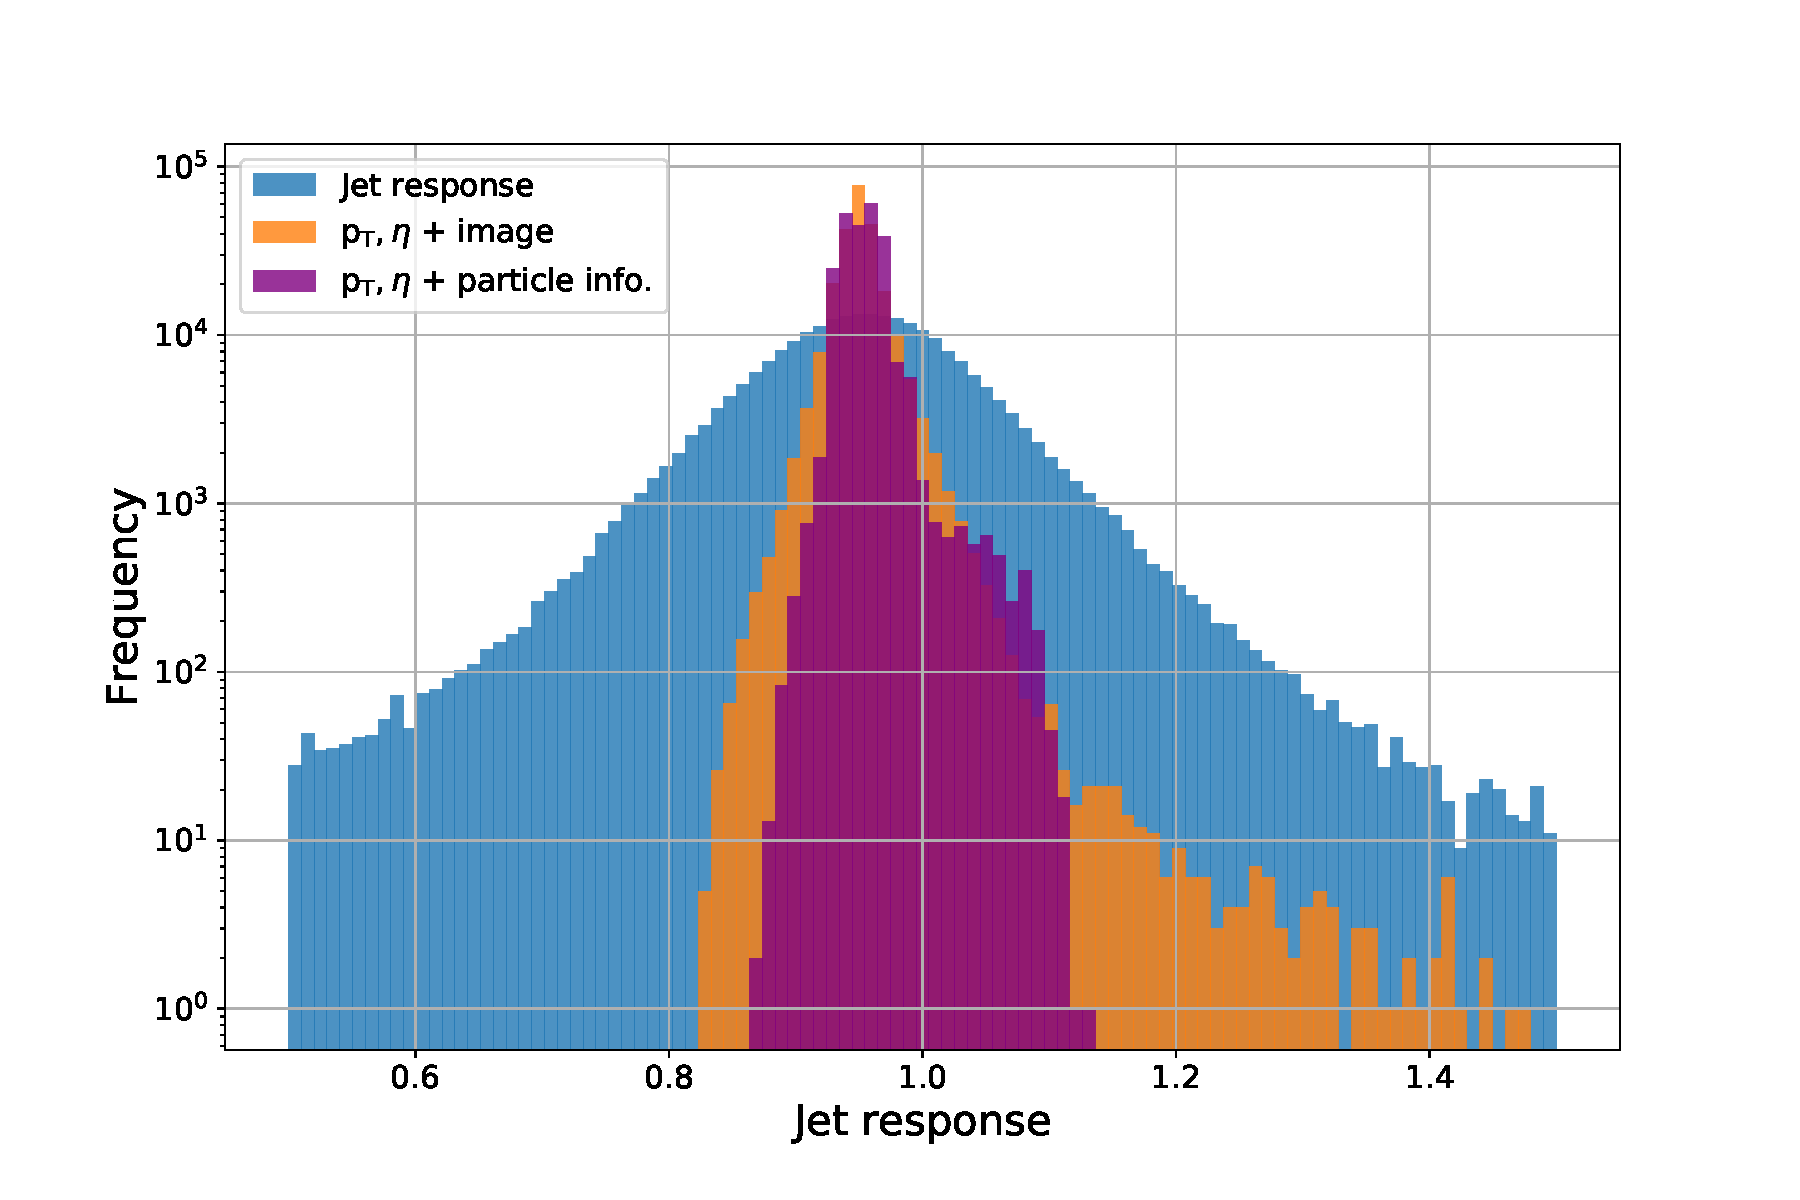
\includegraphics[angle=0,width=0.80\columnwidth]{fig/dnn_prediction.pdf}
\end{center}
\caption{The true jet response distribution (blue), model of the response trained on jet \pT, $\eta$, and jet images (orange), and a model trained on jet \pT, $\eta$, and jet fragmentation information (purple).}
\label{fig:dnn_prediction}
\end{figure}

\end{section}

\begin{section}{Conclusions}

While these results are certainly preliminary and much work is left to do, there is early indication that by encoding the particle-level information of jets through jet images, one can significantly improve the jet response measurement.
This is because these jet images not only include the individual particle information but also the energy and spatial correlations of the jet fragmentation.
This has the potential to help improve both the core and the tail of the jet resolution.

There are, however, many steps necessary before this potential can be realized.
This includes increasing the training set size to $\sim$10 million jets, as well as including pileup effects.
Additionally, a more detailed investigation is needed to understand what the network is learning.
Lastly, this method will have to be validated in data as the details of the jet fragmentation may not be well simulated, and in this case, features developed by training on simulated jets may not correspond to useful features for jets in data.
This can be done through tag-and-probe methods using, for example, phtoon + jets or QCD di-jet events.

\end{section}
